\documentclass[12pt, letterpaper]{article}
\usepackage[utf8]{inputenc}
\usepackage{indentfirst}
\usepackage{graphicx}
\usepackage{setspace}
\usepackage[numbers]{natbib}
\usepackage [autostyle, english = american]{csquotes}
\MakeOuterQuote{"}
\usepackage{layout}
\usepackage[title]{appendix}
\usepackage[justification=centering]{caption}
\usepackage{titlesec}
\usepackage[percent]{overpic}


\begin{document}

\setcounter{secnumdepth}{-1}
\titlespacing*{\section}{0pt}{2\baselineskip}{.33333\baselineskip}
\binoppenalty=\maxdimen
\relpenalty=\maxdimen

%Cover page: 5pts
%Course, subject, name, date
\title{MA348 Numerical Analysis, Thermodynamics}
\author{David Jefts}
\date{February 2, 2019}
\begin{titlepage}
	\centering
	\maketitle
	\centering
	\hfill
	\vfill
\end{titlepage}

\setlength{\voffset}{-0.5in}
\setlength{\headsep}{10pt}

%Introduction: 5pts
%Describe the problem and state objectives
\section{Introduction}
	The goal of this lab is to use various algorithms to estimate the root of a function. In this case, the function was van der Waal's equation of state, ${(P+\frac{a}{v^2})(v-b)=RT}$, where $P$ is the Pressure in atmospheres, $R$ is the Gas Constant for oxygen in atmospheres per mole-Kelvin, $T$ is the temperature in Kelvin, $v$ is the modal volume and ${v=\frac{V}{n}}$, $V$ is the total volume, $n$ is the number of moles of gas present, $a$ is the measure of the average attraction between particles, and $b$ is the volume excluded by a mole of particles. In many chemical engineering models, a very accurate modal volume of an atom or molecule, in this case oxygen,  is required in order to properly construct containment apparatuses for these gases. van der Waal's equation of state is an expansion upon the classic Ideal Gas Law formula, ${PV=nRT}$. Using the relationship ${v=\frac{V}{n}}$, the Gas Law formula used for this lab is $Pv=RT$. In this lab, the values for $R$, $a$, and $b$ are constant and known, $T$ and $P$ change between trials but are known, and $v$ changes relative to the previous variables based on van der Waal's equation.

%Theory-Analysis: 5pts
%State assumptions and develop equations
\section{Theory-Analysis}
	 The function for this lab is van der Waal's equation of state, ${(P+\frac{a}{v^2})(v-b)=RT}$, and the objective is to estimate roots for this function. $v$ is the changing variable, essentially the `$x$' value, so the function must be solved in terms of $v$:

		\begin{center}
			$f(v)=Pv^3-(bP+RT)v^2+av-ab=0$
		\end{center}
	
	This function serves as the main `$f(v)$' function for the remainder of this report. In addition, some of the algorithms used require the derivative and the second derivative of this function:
	
		\begin{center}
			$f'(v) = 3\times Pv^2-2\times (bP+RT)v+a=0$
		\end{center}
		
		\begin{center}
			$f''(v) = 6\times Pv-2\times (bP+RT)=0$
		\end{center}

	
	The Ideal Gas Law formula solved for $v$ is:

		\begin{center}
			$v=\frac{RT}{P}$
		\end{center}

	The only assumptions in this report are the oxygen Gas Constant values for $R$, $a$, and $b$. For this report, $R\approx0.082054$, $a\approx1.360$, and $b\approx0.03183$. Additionally, the Fortran installation used to compute root values is only capable of representing 16 decimal places and is ineffective at representing extremely small numbers due to computer round-off and truncation errors.

%Numerical Solution: 20pts
%Describe the numerical methods used to solve the problem
\section{Numerical Solution}
	This lab was solved using Fortran code to estimate the roots of the function and gnuplot to plot and tabulate the values. Multiple different methods were used, which as a group are colloquially called "open methods." This name comes from the fact that all of the methods work on an "open" set of numbers as opposed to the "bracketing" methods that work only on a set of numbers within a limited range.
	
	Newton's Method (also known as the Newton-Raphson method is an approximation algorithm that uses the tangent line of a function to estimate the root. Starting with a given value, it iteratively uses the function $x_{n+1}=x_n-\frac{f(x_n)}{f'(x_n)}$ until a desired accuracy is reached. This method converges quadratically, making it a very desirable method for quickly calculating the root of a function and it is relatively easy to extend this method to high-order equations and functions. The drawbacks to this method are that the derivative of $f(x)$ has to be recalculated each iteration and the method will completely fail if $f'(x)=0$ at any point during the iteration process.
	
	The Secant Method is an approximation algorithm that uses the secant line of a function to estimate the root. Starting with a given value, it iteratively uses the function $x_{n+1}=x_n-\frac{f(x)\times(x_n-x_{n-1})}{f(x_n)-f(x_{n-1})}$ until a desired accuracy is reached. The Secant Method converges slightly slower than Newton's Method, on the order of ${\approx}1.618$, the Golden Ratio. This method can be implemented easier than the Newton Method since the derivative of $f(x)$ does not need to be calculated, however this method requires two initial points to start and it is not always guaranteed to converge.
	
	The Modified Secant Method is another approximation algorithm that uses the secant line of a function to estimate the root. This method is a modification of The Secant Method detailed above, taking advantage of Newton's difference quotient function to estimate the derivative. It iteratively uses the function $x_{n+1}=x_n-\frac{f(x_n)\times\delta)}{f(x_n+\delta)-f(x_n)}$ until a desired accuracy is reached. The Modified Secant Method converges at the same rate as The Secant Method, while removing the need to define and track two initial points. However it requires a definition of delta ($\delta$) with constraints- if defined too large it may skip over the root, too small and it may never converge in a reasonable amount of time. For this purposes of this lab $\delta=0.01$.
	
	The Modified Newton's Method for Roots of Multiplicity is an approximation algorithm that uses the tangent line of a function and its second derivative to estimate the root. This method iteratively uses the function $x_{n+1}=x_n-\frac{f(x_n)\times f'(x_n)}{(f'(x_n))^2-f(x)\times f''(x_n)}$ until a desired accuracy is reached. Like Newton's Method, this method converges quadratically. Additionally, this method works even if there is a Root of Multiplicity (i.e. the function has two roots of the same value such as $f(x)=x^2-9$. However calculating the second derivative of a function is not always easy.
	
	For the comparison test using $P=10$atm and $T=100$K and starting numbers of $x_{n+1}=3, x_n=4,$ and $x_{n-1}=5$:
	
	\begin{center}
		Newton's Method converged in 4 iterations
		
		The Secant Method converged in 6 iterations
		
		The Modified Secant Method converged in 5 iterations
		
		The Modified Newton's Method for Roots of Multiplicity converged in 6 iterations
	\end{center}

%Results and Discussion: 45pts
%Tabulate and plot the results, compare results, and discuss the accuracy of results
\section{Results and Discussion}
    	Firgure~\ref{fig:error} in Appendix A is a graph of the error during each iteration of each algorithm, where each line represents one of the above-mentioned estimation methods, the x-axis is the number of iterations and the y-axis is the error. In this graph scenario $P=10atm$ and $T=300K$. This graph seems to indicate that Newton's Method both starts with a smaller error and converges towards the desired value faster. The other methods all converged upon the same value, but were slower, less efficient, and/or unnecessarily complicated (as in the case of the Modified Newton's Method for Roots of Multiplicity since this function does not have any roots with multiplicity). When compared with the Ideal Gas Law however, they all reached a Modal Volume about $0.2\frac{m^3}{mol}$. The cause of this discrepancy is most likely due to the corrections the van der Waal's equation makes to the Ideal Gas Law formula by observing and allowing for the fact that gas molecules attract each other (noted by the variable $a$ in his equation) and the volume of each individual mole of gas (noted by the variable $b$ in his equation).
	
%Conclusions: 20pts
%Comment on the efficiency of the solvers
\section{Conclusions}
	Newton's Method appears to be the most efficient method without sacrificing any error or simplicity, in the future that may not always be the case though, depending on the function, how it curves, and what its roots are. If this were to be done by hand the most accurate and efficient way would be Newton's Method, however the other methods do not converge at a significantly slower rate when using a tolerance of $10^{-6}$. There are many other ways to optimize the estimation this function however, the methods of finding roots detailed in this report are just a handful from a plethora of various solvers and algorithms that accomplish the same task. 

\pagebreak
	
%Appendices
%Include listings of the source codes, include printed copies of the output files
\appendix
	\section{Appendix A}
            		\begin{figure}[htp]
            			\centering
            			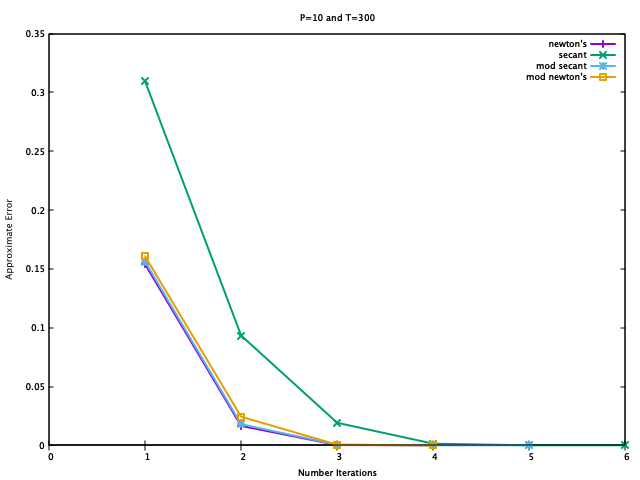
\includegraphics[width=1.0\linewidth]{ErrorGraphs.png}
            			\caption{Graph of the error over time for each algorithm}
            			\label{fig:error}
            		\end{figure}
	\pagebreak

	\section{Appendix B}
		Graphs of each combination of Pressure/Temperature. The green line represents the graph of the Ideal Gas Law at the given Pressure and Temperature (enumerated in the title of each graph) while the purple line represents the Newton's Method Estimation function on the interval. $v$ is the modal volume estimated by Newton's Method.
		
		%1 atmosphere of Pressure
		\begin{figure}[htp]
			\centering
			\begin{overpic}[width=0.5\textwidth]{1&300.png}
				\put (15,35) {\huge$\displaystyle v=24.592799$}
			\end{overpic}
			\caption{$P=1atm$, $T=300K$}
		\end{figure}

		\begin{figure}[htp]
			\centering
			\begin{overpic}[width=0.5\textwidth]{1&500.png}
				\put (15,35) {\huge$\displaystyle v=41.025704$}
			\end{overpic}
			\caption{$P=1atm$, $T=500K$}
		\end{figure}

		\begin{figure}[htp]
			\centering
			\begin{overpic}[width=0.5\textwidth]{1&700.png}
				\put (15,35) {\huge$\displaystyle v=57.445966$}
			\end{overpic}
			\caption{$P=1atm$, $T=700K$}
		\end{figure}
		
		%10 atmospheres of Pressure
		\begin{figure}[htp]
			\centering
			\begin{overpic}[width=0.5\textwidth]{10&300.png}
				\put (15,35) {\huge$\displaystyle v=2.438403$}
			\end{overpic}
			\caption{$P=10atm$, $T=300K$}
		\end{figure}

		\begin{figure}[htp]
			\centering
			\begin{overpic}[width=0.5\textwidth]{10&500.png}
				\put (15,35) {\huge$\displaystyle v=4.101629$}
			\end{overpic}
			\caption{$P=10atm$, $T=500K$}
		\end{figure}

		\begin{figure}[htp]
			\centering
			\begin{overpic}[width=0.5\textwidth]{10&700.png}
				\put (15,35) {\huge$\displaystyle v=5.752097$}
			\end{overpic}
			\caption{$P=10atm$, $T=700K$}
		\end{figure}

		%100 atmospheres of Pressure
		\begin{figure}[htp]
			\centering
			\begin{overpic}[width=0.5\textwidth]{100&300.png}
				\put (15,35) {\huge$\displaystyle v=0.226358$}
			\end{overpic}
			\caption{$P=100atm$, $T=300K$}
		\end{figure}

		\begin{figure}[htp]
			\centering
			\begin{overpic}[width=0.5\textwidth]{100&500.png}
				\put (15,35) {\huge$\displaystyle v=0.411614$}
			\end{overpic}
			\caption{$P=100atm$, $T=500K$}
		\end{figure}

		\begin{figure}[htp]
			\centering
			\begin{overpic}[width=0.5\textwidth]{100&700.png}
				\put (15,35) {\huge$\displaystyle v=0.584196$}
			\end{overpic}
			\caption{$P=100atm$, $T=700K$}
		\end{figure}

	\clearpage
	
	\section{Appendix C}
		\begin{figure}[h]
			\centering
			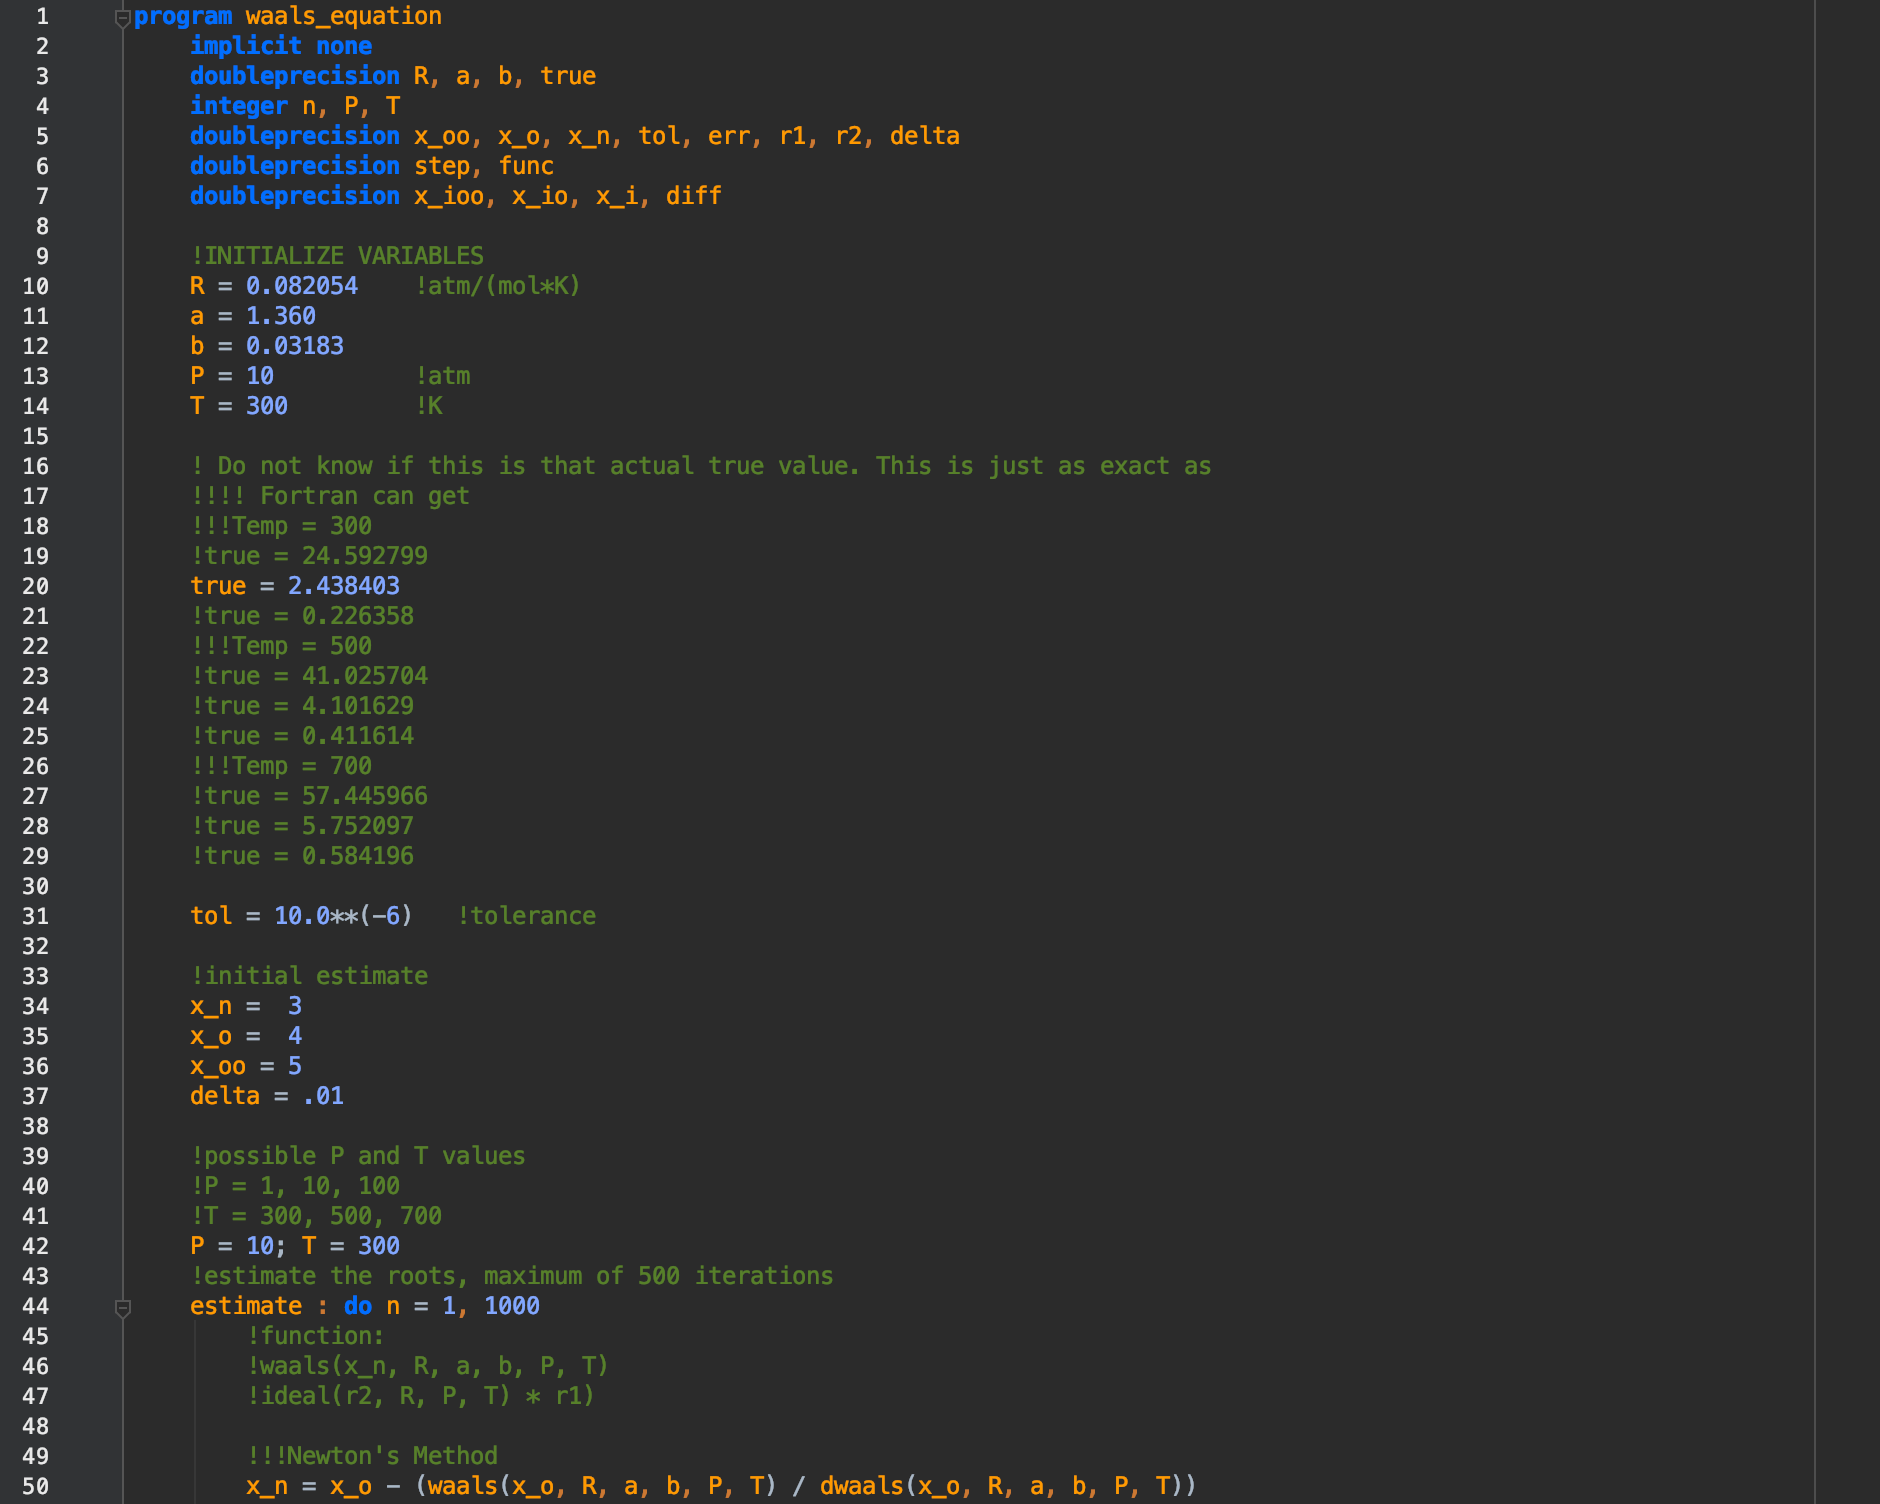
\includegraphics[width=.864\linewidth]{waalsCode0.png}
		\end{figure}
		\begin{figure}[h]
			\centering
			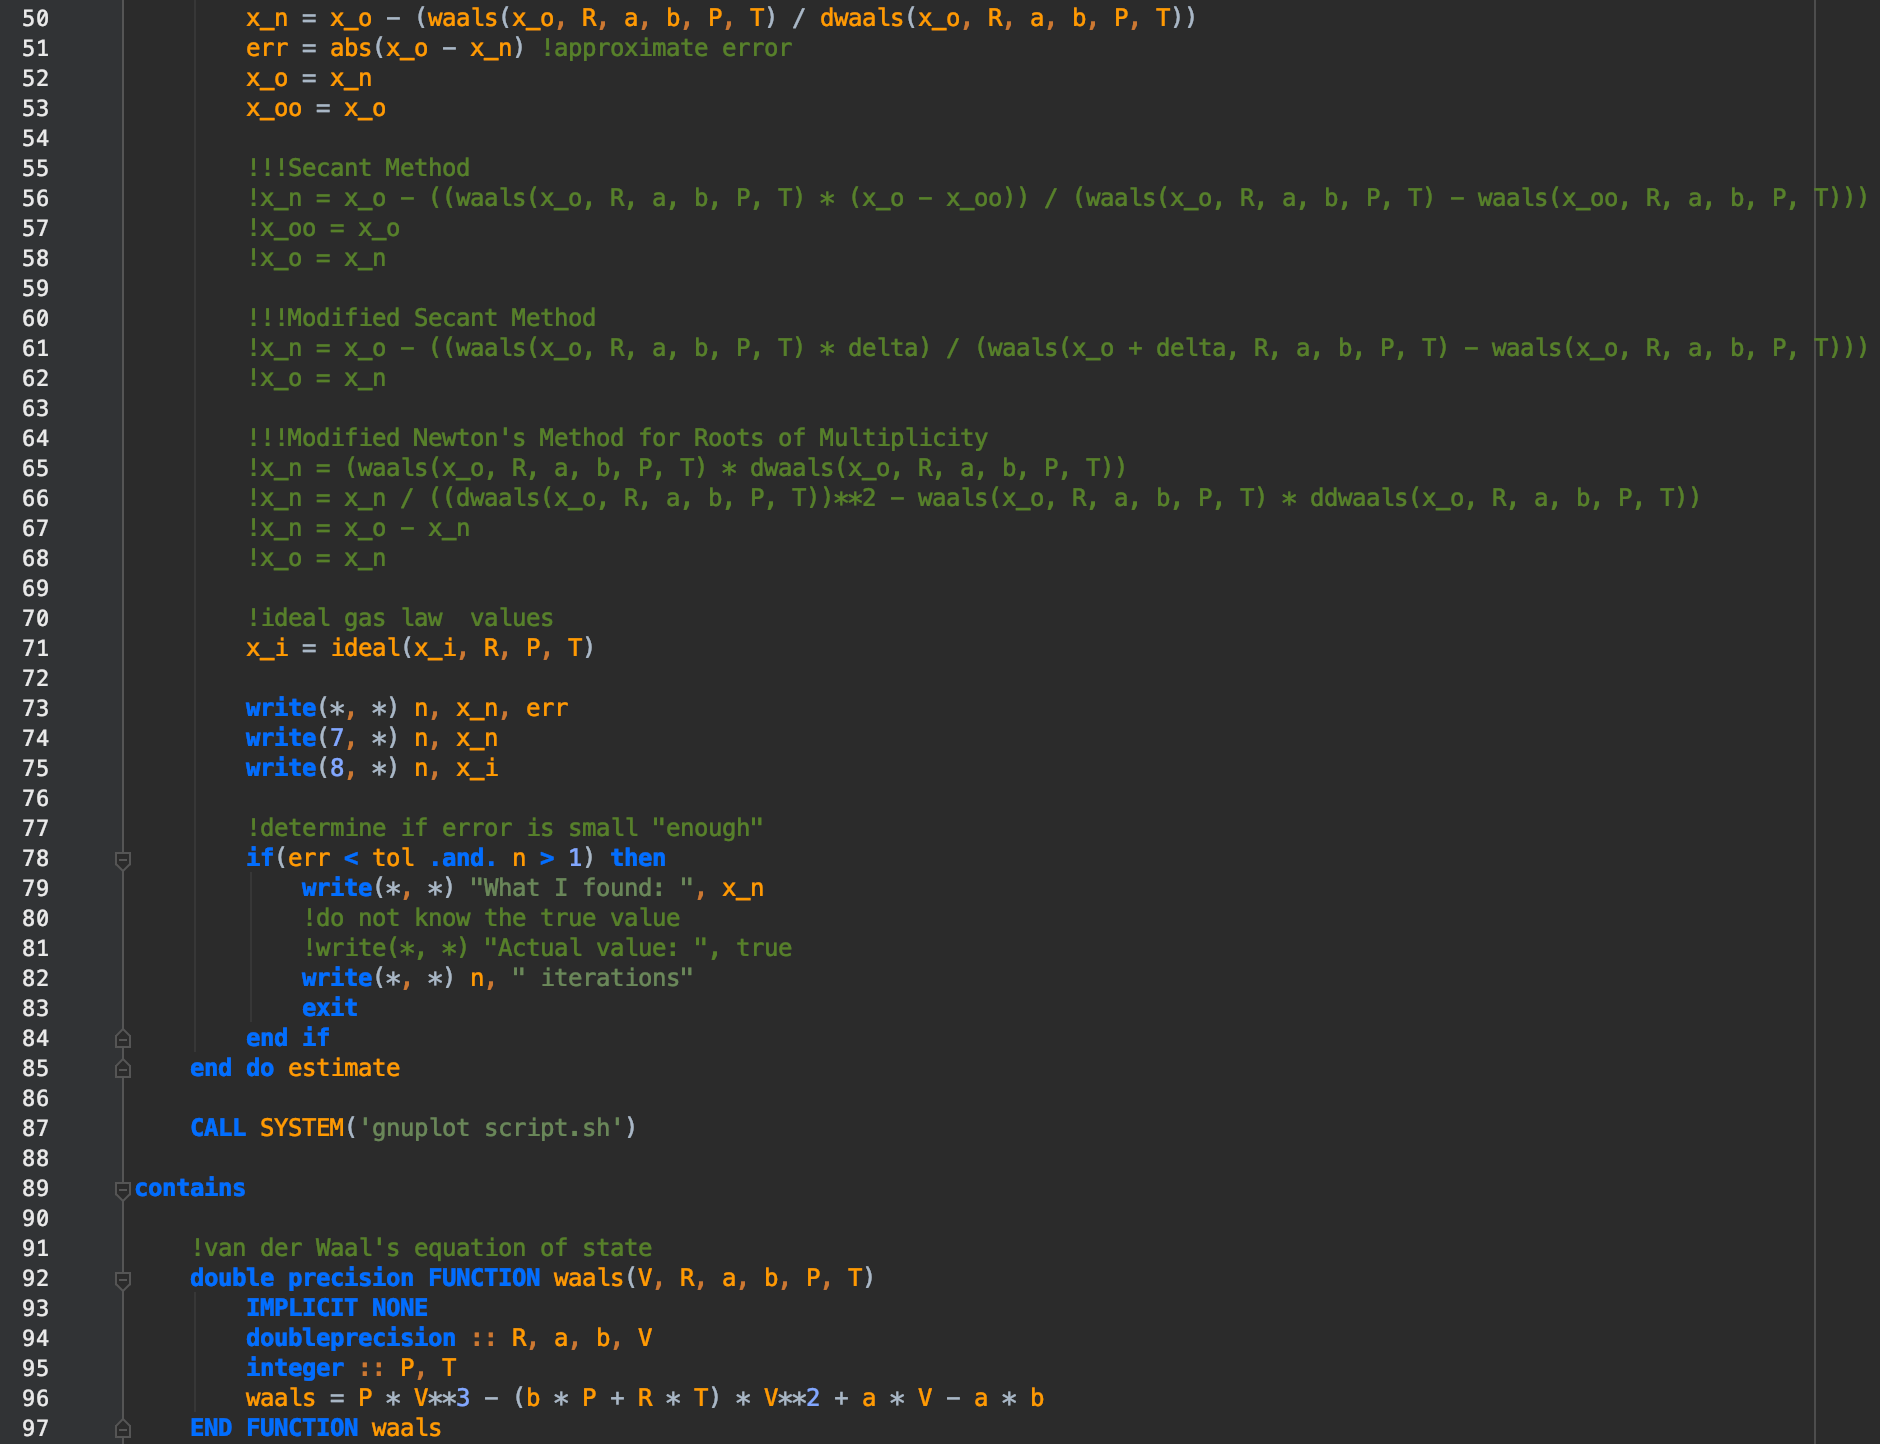
\includegraphics[width=\linewidth]{waalsCode1.png}
		\end{figure}
		\begin{figure}[h]
			\centering
			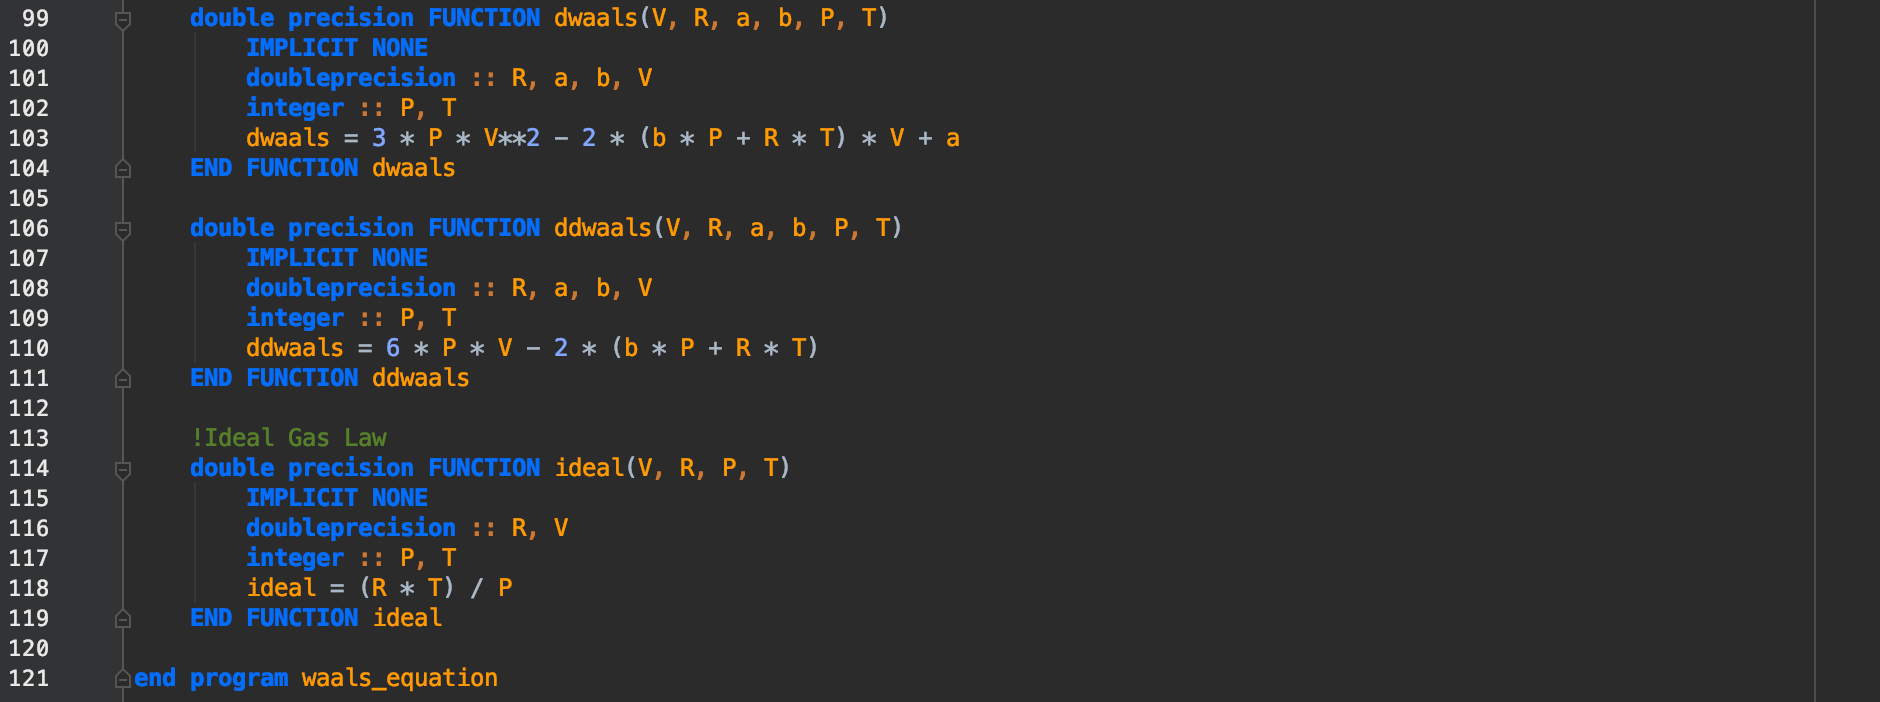
\includegraphics[width=\linewidth]{waalsCode2.png}
		\end{figure}
		\begin{figure}[h]
			\centering
			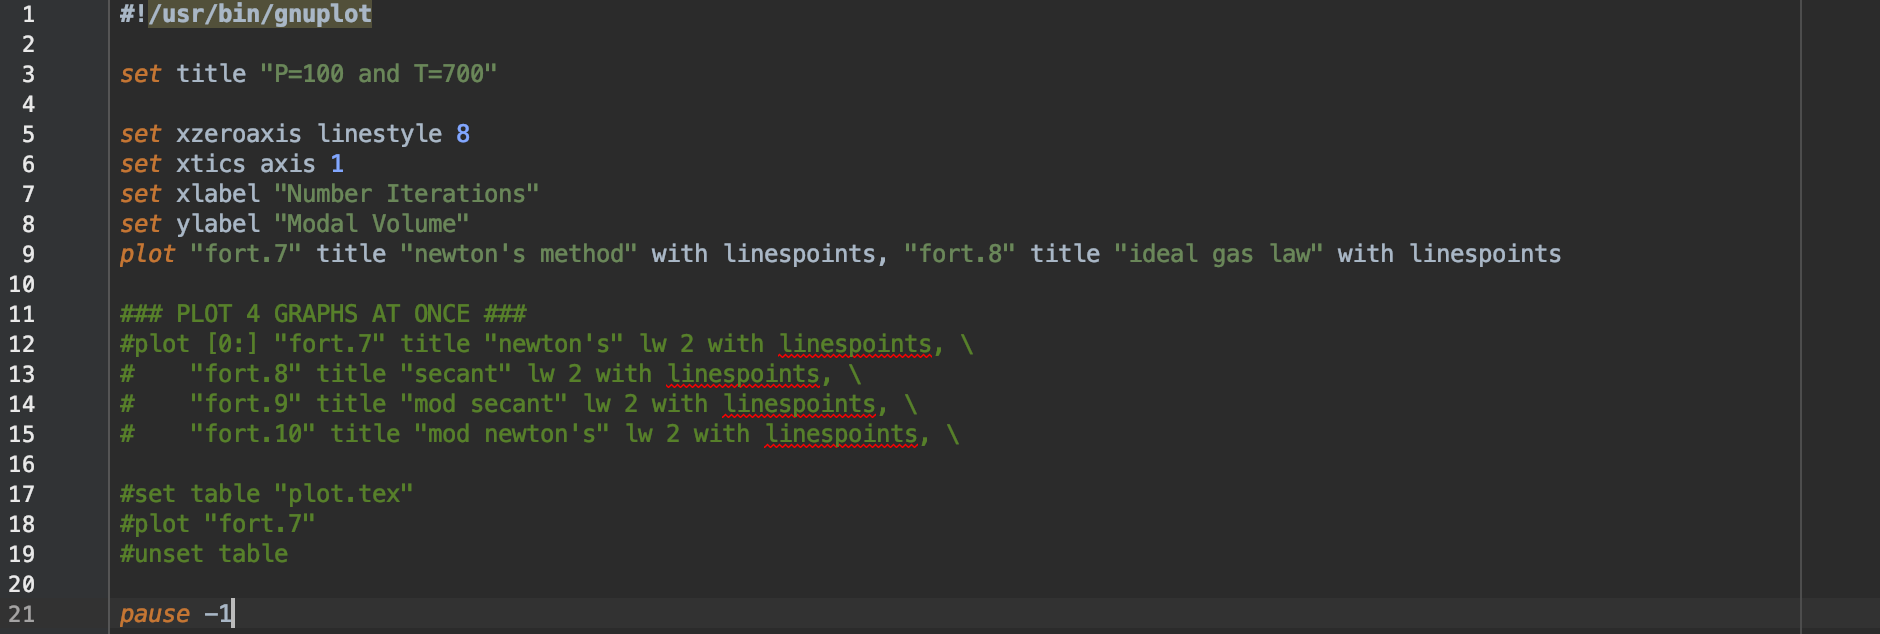
\includegraphics[width=\linewidth]{gnuplotscript.png}
		\end{figure}


\end{document}
